%Préambule du document :
\documentclass[12pt, a4paper]{book}
%\usepackage[latin1]{inputenc} 
\usepackage[utf8]{inputenc} % accents
\usepackage{gensymb} % degree symbol ° (\degree)
\usepackage[T1]{fontenc} % | "`pipe"' character
\usepackage{graphicx}
\usepackage{titling}
\usepackage{amssymb} 
\usepackage{minitoc} % chapter's tocs
\usepackage{authblk} % author affiliations
\usepackage{fancyhdr} % modify the headers
\usepackage{tabularx} % tables not larger than A4
\usepackage[table]{xcolor} %colors inside the tables
\usepackage{float}
\usepackage{multicol} % multiple columns in some sections
\usepackage[inner=2cm,outer=2cm]{geometry} %A4 margins
\usepackage{siunitx}
\usepackage[labelfont=bf, margin=0.5cm]{caption} % for figure captions in minipages
\usepackage{hyperref} %link references (toc, citations) inside document
\usepackage{natbib} % to cite with parentheses and plain text et only year if you please...
\usepackage{amsmath}
 \usepackage{fixltx2e} % allows overrightarrow to be in caption
 \MakeRobust{\overrightarrow}




\bibliographystyle{plainnat} % reference style
\renewcommand{\bibname}{References} %Rename "`bibliography"' => "`references"'

\hypersetup{
    colorlinks,
    citecolor=brown,
    filecolor=green,
    linkcolor=red,
    urlcolor=blue
}
\hypersetup{linktocpage}


\pagestyle{fancy}
\fancyhead{}
\fancyfoot{}
\fancyhead[RO,LE]{\thepage}
\fancyhead[LO]{\leftmark}
\fancyhead[RE]{\rightmark}
\setcounter{tocdepth}{1} % we only want chapters and sections in toc
\setcounter{minitocdepth}{2} %we want sections and subsections in chapters' minitocs

\pretitle{%
  \begin{center}
  
  
\includegraphics[width=17cm]{../Logo_software.png}\\[\bigskipamount]
}
\posttitle{
\\
  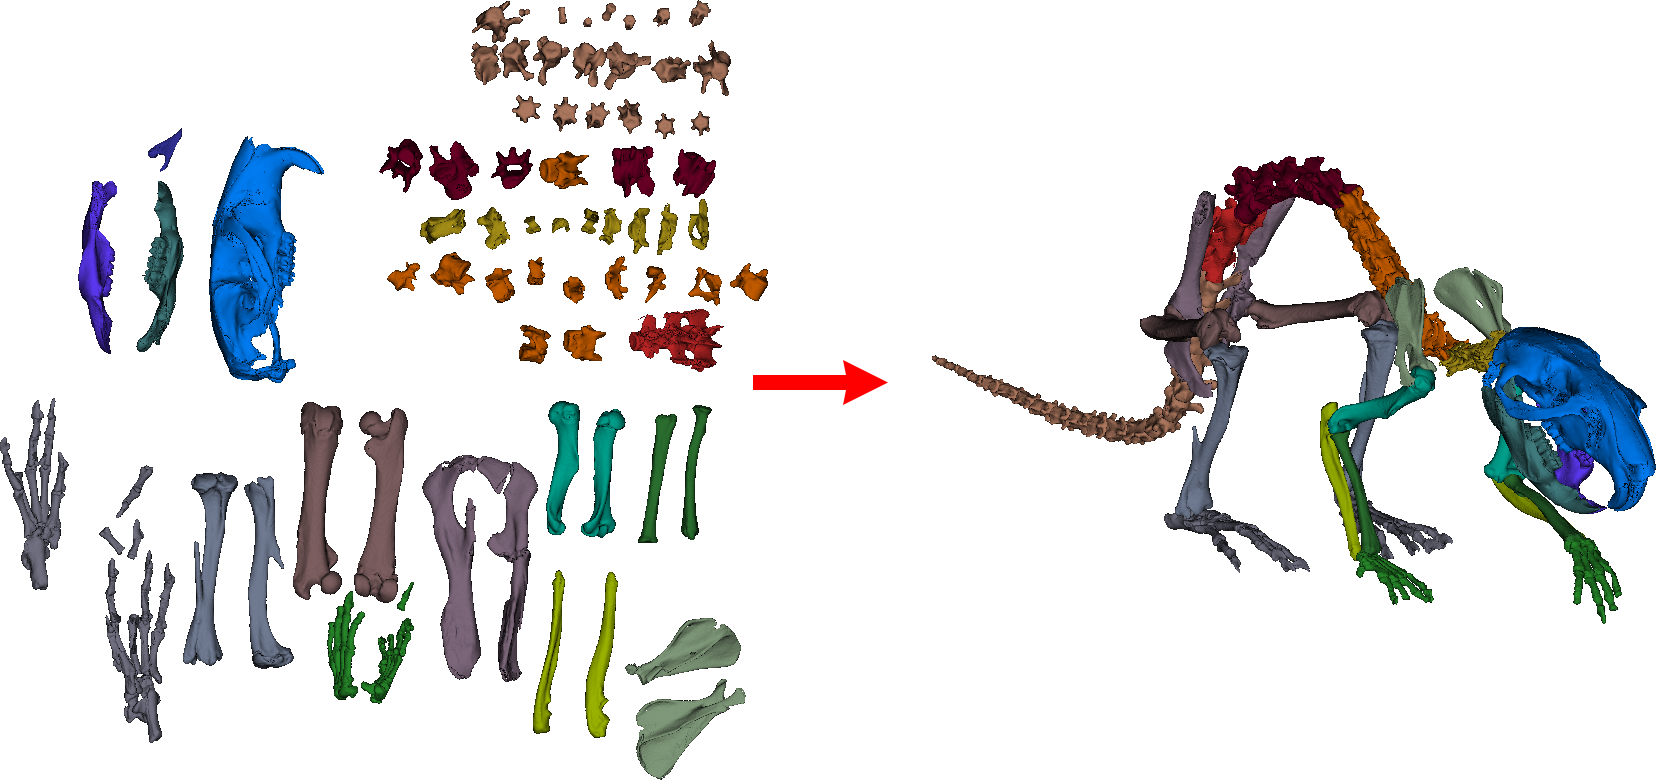
\includegraphics[width=6.5cm]{tutorial03.png}\\[\bigskipamount]
\end{center}}

%\postdate{
%
\includegraphics[width=15cm]{logo_affiliations.png}
%}

\title{MorphoDig Tutorials\\Tutorial 03: working with many surface objects.}



%\titlepicture[width=13cm]{Logo_software.png}
\author{Renaud LEBRUN}
\affil{Institut des Sciences de l'Evolution, Université de Montpellier, France}
\date{\today} 

\def\chaptername{Tutorial}
\setcounter{chapter}{2}
%Corps du document :
\begin{document}

\dominitoc	

\maketitle


\tableofcontents

\chapter{Working with many surface objects}
\addstarredchapter{Working with many surface objects}

\markboth{Working with many surface objects}{}

\minitoc 
Tutorial 03 includes:
\begin{itemize}
\item A series of 74 .vtk surface files, each representing a bone belonging to \textit{Canariomys bravoi}
\item Two series of 74 .pos files (to orientate and position each bone)
\item Two .ntw (project) files. The first one to open each bone in initial orientation/position. The second one to opean each bone in anatomical orientation.
\item One .ori (orientation helper labels) file 
\item The present .pdf document
\end{itemize}

Before using this tutorial, please download and read MorphoDig User Guide.


\section{About the present reconstruction}
\subsection{About the specimens}
The present three-dimensional reconstruction of the skeleton of the giant rat of Tenerife (Canary
Islands, Spain) was obtained by computerized microtomography reconstruction. Two distinct specimens
were used in this reconstruction, TFMCV872 and TFMCV873 (Museo de la Naturaleza y el
Hombre, Santa Cruz). TFMCVF872 is an almost complete but disarticulated skeleton of \textit{C. bravoi}. As
mandibles and skull of this specimen were not well preserved, a complete cranium of \textit{C. bravoi} (TFMCVF873)
was added to this reconstruction. The reconstruction of this fossil was published in Michaux et al. (\citep{MichauxJ2012}) and the 3D model was disseminated  in Michaux et al. (\citep{MichauxJ2015}).\\


\subsection{Completeness}
Murinae rodents observed by Owen (\citep{Owen1853}) always possess a total amount of 19 thoraco-lumbar
vertebrae, most often divided in 13 thoracic and 6 lumbar vertebrae (he also observed at least one
specimen of \textit{Rattus norvegicus} possessing 12 thoracic and 7 lumbar vertebrae). This number of 19
thoraco-lumbar vertebrae is observed very often in mammals and is thought to be a plesiomorphic
condition for eutherians and metatherians mammals (for a review, see for instance Sánchez-Villagra
et al., \citep{SanchezVillagra2007}). The present fossil of C. bravoi exhibits a number of 17 thoraco-lumbar vertebrae, so
there is a high probability that 2 vertebrae (either 1 thoracic and 1 lumbar, or 2 lumbars) are missing.
Furthermore, the number of caudal vertebrae in Murinae rodents observed by Owen (\citep{Owen1853}) is
often greater than the 21 presented in this reconstruction The present reconstruction of Canariomys
bravoi does not take into account these potentially missing thoraco-lumbar and caudal vertebrae, and
you may propose a new reconstruction based on your own observation or Murinae rodents.

\section{Tutorial}
		Download and unzip the files associated to this tutorial.
\subsection{Opening surfaces.}

Download and unzip the 3D files associated to this tutorial. Open MorphoDig.

	You may open the enclosed .vtk surface files (File -> Surface -> Open Surface) or one by one, but as there are 74 surfaces, this is time consuming. MorphoDig offers two faster alternatives.\\
You may drag and drop all selected files at once in the 3D main window (see Fig. \ref{drag_and_drop}-A p.\pageref{drag_and_drop}).\\
You may also open all selected files at once when clicking on the "open" (
\includegraphics[scale=0.03]{../images/03/open_data.png}) button inside the main window (or press "CTRL +O").\\

\begin{figure}
  \centering
  \includegraphics[scale=0.3]{dag_and_drop.png} 
	\caption{Opening many surfaces at once and changing their color.  A: you may drag and drop all 74 surfaces surface at once inside the main 3D window.  B: you may then browse through the 74 opened surfaces via the "Edit first selected surface" window and change the solid color of each bone.}
\label{drag_and_drop}
 
\end{figure}


\subsection{Setting the position of each bone.}

You may interact with selected objects (those which are drawn grey) in different ways (see MorphoDig user guide for further explanations).\\


By default (\includegraphics[scale=0.7]{../images/06/camera/move_cam2.png}), the camera rotates around the center of mass of all opened objects. This behavior is useful when the center of mass of an object (or of several ones) is far from the origin of the coordinate system. But by pressing the camera button (\includegraphics[scale=0.7]{../images/06/camera/move_cam2.png} -> 
\includegraphics[scale=0.7]{../images/06/camera/move_cam.png}), the camera will revolve around the center of the coordinate system (x=0, y=0, z=0).  The display grid is drawn using different colors depending on the camera rotation center (see Fig. \ref{grid_color} p.\pageref{grid_color}).


In order to help positioning surfaces in a biologically-relevant manner, 6 predefined camera positions are defined:\\

\includegraphics[scale=0.7]{../images/06/camera/camera_right.png} view object from right side \\

\includegraphics[scale=0.7]{../images/06/camera/camera_left.png} view object from left side\\

\includegraphics[scale=0.7]{../images/06/camera/camera_front.png} view object from front side (default camera position)\\

\includegraphics[scale=0.7]{../images/06/camera/camera_back.png} view object from back side\\

\includegraphics[scale=0.7]{../images/06/camera/camera_above.png} view object from above\\

\includegraphics[scale=0.7]{../images/06/camera/camera_below.png} view object from below\\

In "object interaction mode(
\includegraphics[scale=0.7]{../images/04/move_mode.png})", selected objects can be translated and rotated using the mouse left and middle buttons (in landmark 
\includegraphics[scale=0.7]{../images/04/Landmarks2.png} and camera  
\includegraphics[scale=0.7]{../images/04/camera_mode.png} selection modes, you also need to maintain ``CTRL" button pressed while dragging the left mouse button to achieve rotation and translation of selected objects). Alternatively, you may also use the "yellow sliders" located on the right side of the 3D main window to accomplish rotation and translation of selected objects. Rotation is achieved around the global center of mass of all currently selected objects, which is convenient to rotate groups of bones (such as: all bones belonging a given anatomical unit such as the limbs, the head, the tail etc.).\\
\begin{figure}
  \centering
  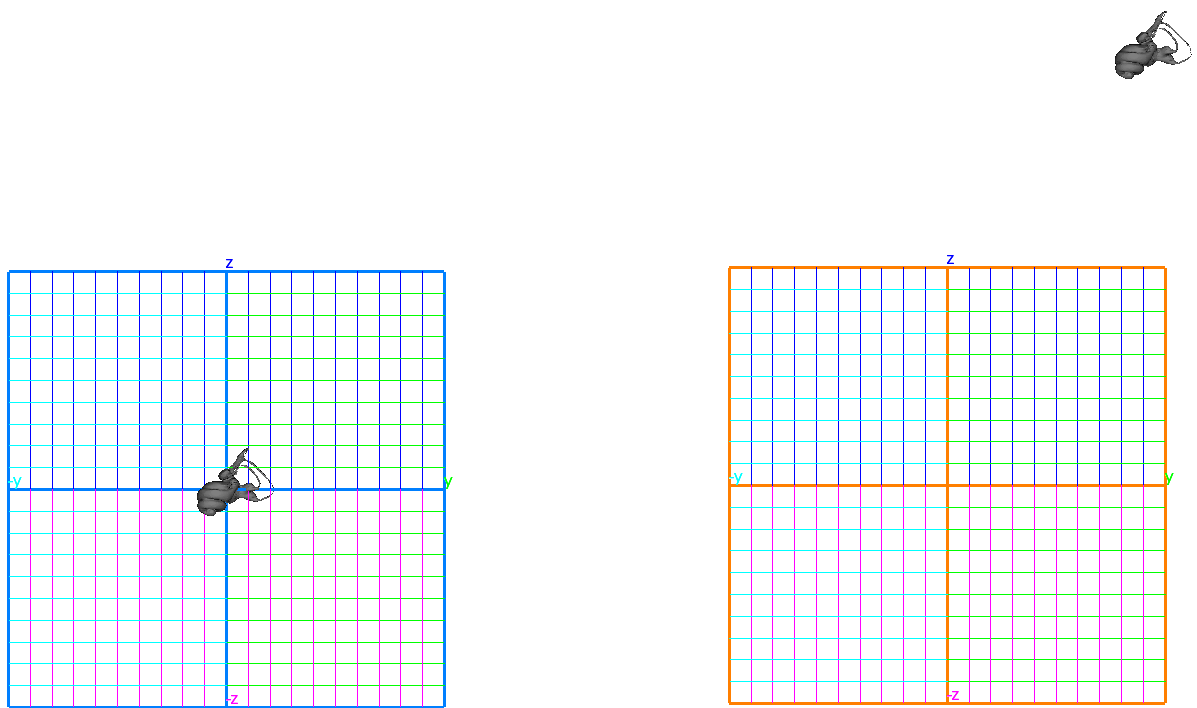
\includegraphics[scale=0.3]{grid.png} 
	\caption{Grid display color.  Left: when the camera revolves around the center of mass of all opened objects, the grid has a blue outline. Right: when the camera revolves around the origin of the coordinate system (x=0, y=0, z=0), the grid outline is displayed in orange.}
\label{grid_color}
 
\end{figure}

.\\
All opened surfaces can be unselected by pressing "CTRL +D", or selected by pressing "CTRL +A". All selected objects can be deleted by pressing "Del".

\begin{figure}
  \centering
  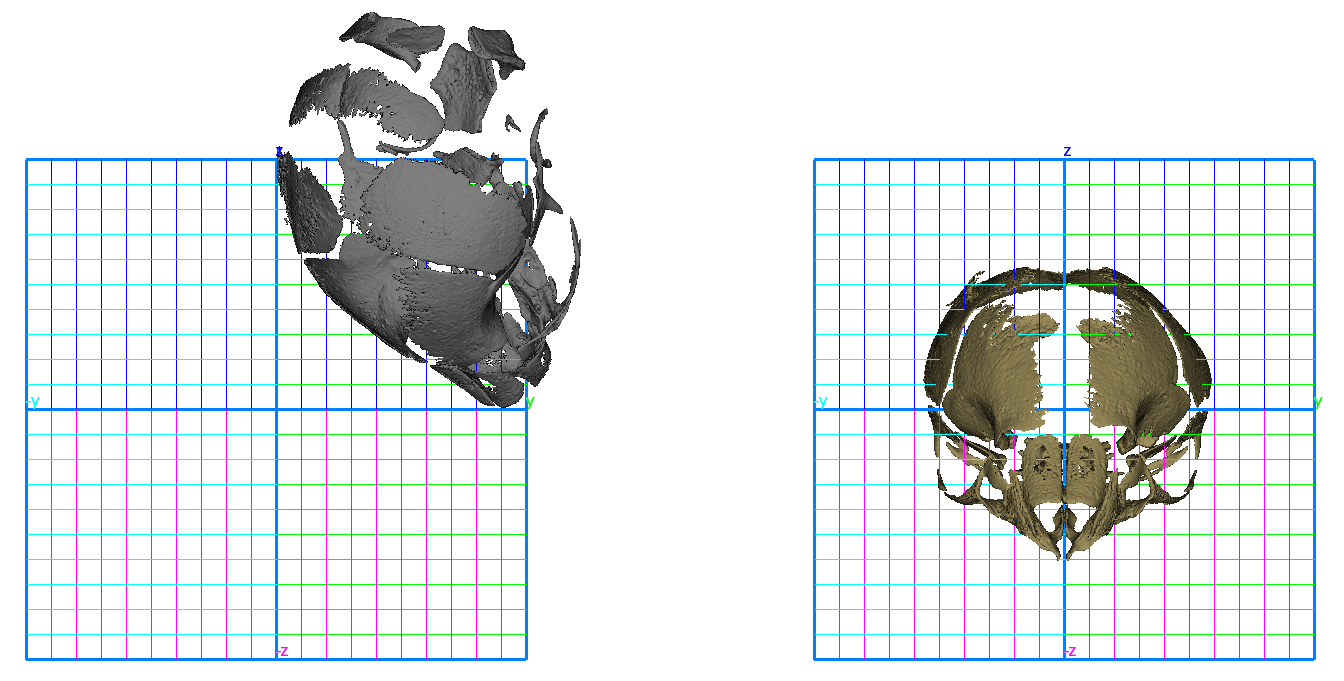
\includegraphics[scale=0.3]{pos.png} 
	\caption{A convenient way to orientate right inner ears.  Left: when viewed from the front side, the lateral canal is placed horizontally. Right: when viewed from above, the cochlea points towards the bottom right-hand of the screen, and the lateral canal towards the top left-hand of the screen.}
\label{orientation}
 
\end{figure}


\subsection{Mouse inner ear project file}
The present tutorial contains a project .ntw file, which may be useful to directly open the right inner ear
 in a convenient position, to make it transparent and to give it a color. First, delete all currently opened objects
(press "CTRL+A", then press "Del"). Then open the enclosed .ntw file (File -> Open Project, then select
"Mouse\_right\_ear.ntw"). Once loaded, the right inner ear surface is opened, is given the position
enclosed in the "Mouse\_right\_ear.pos" file, a color and a transparency. Note that the newly opened
surface is unselected.\\

\subsection{Mouse inner ear curve file}
3D Curves are constructed in MorphoDig using 2 series of landmarks : a series of "curve node" landmarks (
\includegraphics[scale=0.7]{../images/04/curve_nodes.png}),
and a series of "curve handle" landmarks (
\includegraphics[scale=0.7]{../images/04/curve_handles.png}). The numbers of curve nodes and curve handles should be equal. The Mouse\_right\_ear.stv contains the 3D coordinate of a series of  33 "curve node" and 33 "curve handle" landmarks. You can load it (File->Curves->Load MorphoDig Landmark/Curve file(.STV), or drag and drop this file directly in the 3D main window).\\

You may consider to change the way landmarks and curve handles are rendered in the "Landmark and flag options" window (Edit->Edit landmark and flag rendering options ). In this tutorial, you may display landmarks as spheres and to set their rendering size to 0.05 mm.\\

\subsection{Mouse inner ear .ori file}
The present tutorial contains a .ori file, which contains orientation labels for the coordinate system
orientation helper. You can load this file the enclosed .ori file ("File->Orientation helper labels -> Open Orientation labels", then select
"Mouse\_right\_ear.ori"). Once loaded, the system coordinate orientation helper will show the following
labels :\\
+z axis : superior\\
-z axis : inferior\\
+y axis : medial\\
-y axis : lateral\\
+x axis : proximal\\
-x axis : distal\\
You may set your own orientation axis labels with the “Edit orientation labels” window (Edit-> Edit orientation labels)

\section{Curve digitization with MorphoDig}


When digitizing curve node and curve handle landmarks, I recommend to press "
\includegraphics[scale=0.7]{../images/04/Landmarks2.png}" to activate the "Landmark mode". When active, only landmarks can be selected/unselected via right mouse button drag/click. \\

As stated earlier, two series of landmarks involved into the construction of 3D curves can be set with MorphoDig: "curve node" and "curve handle" landmarks.
Press "
\includegraphics[scale=0.7]{../images/04/curve_nodes.png}" to activate curve node landmark setting mode, “
\includegraphics[scale=0.7]{../images/04/curve_handles.png}” to activate curve handle landmark setting mode mode.\\


Landmarks can be set on surfaces by pressing "L" + left mouse click. If a single landmark is selected, its position can be moved
on another part of the surface by pressing "L" + right mouse click (nothing happens if no landmark
is selected or if more than one landmark are selected). Also, you may need to move landmarks away
from the object's surface (for instance when you want to place a landmark at the centere of a semicircular canal):
once selected, a landmark position can be moved by using the usual mouse (CTRL + middle click + mouse drag) and GUI controls.\\

You may sometimes need to reorder landmark objects. 
Selected curve node/handle landmarks can be reordered
using the following buttons. Clicking on 
\includegraphics[scale=0.7]{../images/06/objects/move_up.png} will increase (= move down in list, if possible) the landmark number of all selected landmarks. Clicking on 
\includegraphics[scale=0.7]{../images/06/objects/move_down.png} will decrease (=move up in list, if possible) the landmark number of all selected landmarks. 

\subsection{Digitization strategy}
\begin{figure}
  \centering
  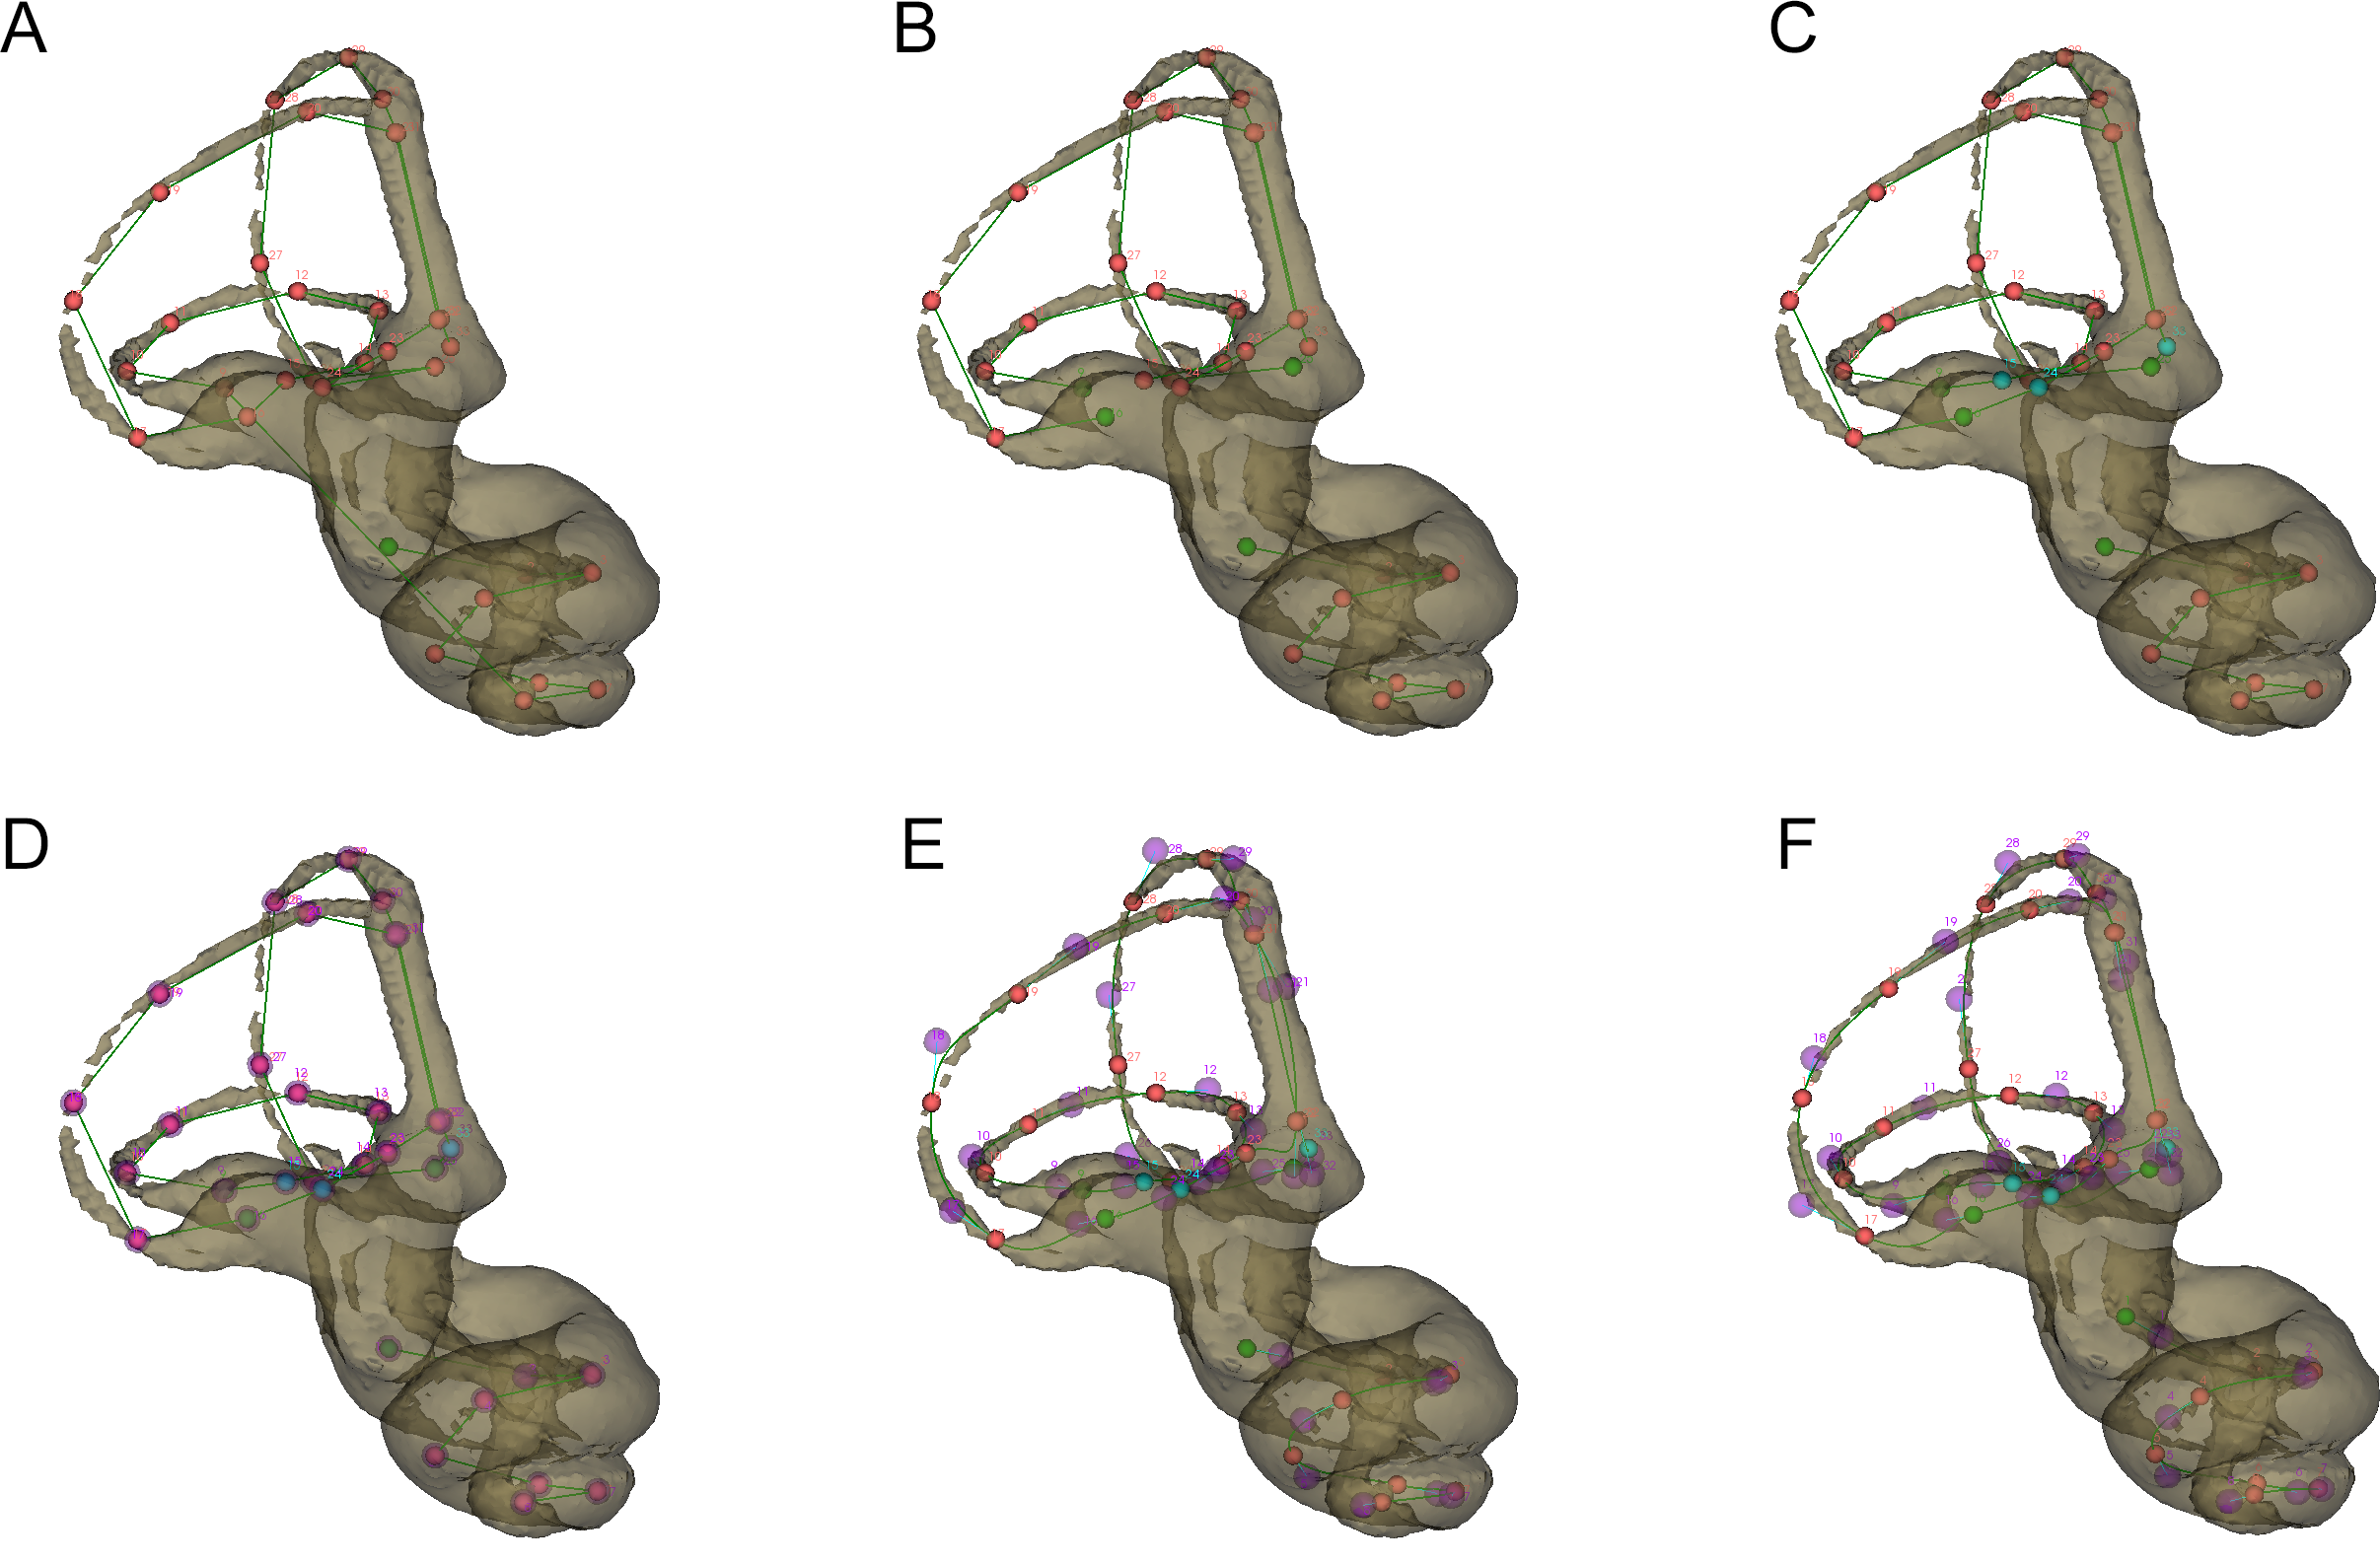
\includegraphics[scale=0.2]{curve_digitization.png} 
	\caption{Curve digitization strategy with MorphoDig. \textbf{A:} digitization of curve node landmarks. \textbf{B:} Nodes 9, 16 and 25 are now starting nodes (dark green). \textbf{C:} Nodes nodes 15, 24 and 33 are connected to their preceding starting node to close the three semicircular canals. \textbf{D:} Curve node coordinates were saved  as a .ver file, and are loaded in a second step as handle landmarks (violet). \textbf{E:} Curve handles were displaced automatically. \textbf{F:} several curve nodes and curve handles were displaced manually (last and most time consuming step)}
\label{curve_digitization}
 \end{figure}
To digitize curves on an inner ear, I recommend to use the following 3 steps strategy:
\subsubsection{1) Digitize a series of "curve node" landmarks, and define curve starting points}
As curves pass through curve node landmarks, these curve nodes will endorse the role of the "skeleton" of all curve segments. In the present tutorial, a series of 33 "curve node" landmarks was set inside the cochlea, the lateral semicircular canal, on the anterior and posterior semi-circular canals (Fig. \ref{curve_digitization}-A p.\pageref{curve_digitization}). You may load the enclosed .ver file (File->Curves->Open Curve Node Landmarks-> Mouse\_right\_ear.ver).\\

Then select landmarks 9, 16 and 25, and define them as curve starting points (Landmarks->Selected curve node and curve handle landmarks-> Normal nodes (red): define as starting nodes (dark green)). The consequence of this action is that the series of 33 landmarks will contain four
curves : one defining the cochlea, and one for each of the 3 semi-circular canals (Fig. \ref{curve_digitization}-B p.\pageref{curve_digitization}).\\

As an option, you may select curve nodes 15, 24 and 33 and connect them to their preceding starting
nodes (Landmarks->Selected curve node and curve handle landmarks-> Normal nodes (red): connect
to preceding starting nodes (cyan)). The consequence of this action is that the curves representing
the 3 semi-circular canals will be closed (Fig. \ref{curve_digitization}-C p.\pageref{curve_digitization}).\\
Save the current series of landmarks (File->Curves->Save Curve Node Landmarks).

\subsubsection{2) Load curve handles and modify their position semi-automatically}
- Load curve handles (File->Curve->Open Curve Handle Landmarks-> then select the file you just created
in the preceding step, here chose the "Mouse\_right\_ear.ver" file, Fig. \ref{curve_digitization}-D p.\pageref{curve_digitization}).\\
- Select all the curve handles (the easiest way to achieve this is to press “CTRL +A”, to select all currently
opened objects).\\
- Move curve handles semi-automatically (Landmarks->Selected curve node and curve handle landmarks-> Move curve handles semi-automatically). Chose a value of 25\%, press "Ok" (Fig. \ref{curve_digitization}-E p.\pageref{curve_digitization}), and then unselect all objects (CTRL+D).\\

\subsubsection{3) Modify curve handles and normal landmarks manually}
The last step (and probably the hardest one) is to move manually the curve nodes and curve handles in order to make the curves follow the geometry of the studied structures (Fig. \ref{curve_digitization}-F p.\pageref{curve_digitization}).

\subsection{Saving and exporting curves}
\begin{figure}
  \centering
  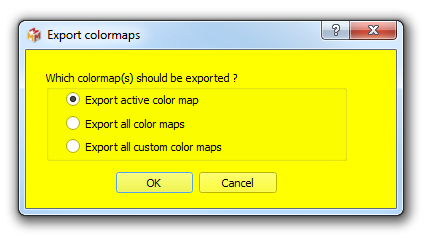
\includegraphics[scale=0.3]{export.png} 
	\caption{Exporting curves. \textbf{A:} curve digitization involving with 33 curve node and 33 curve handle landmarks. \textbf{B:} each curve segment was exported as 20 equidistant semi-landmarks inside a .ver file. These equidistant semi-landmarks are those used in geometric morphometric analyses.}
	\label{export}
 
\end{figure}
To save all digitized curves, go in “File->Curves” and either save curve nodes and curve handles inside a .STV (recommended) or .CUR file.\\ 
To export all digitized curve segments into series of equidistant semi-landmarks (these latter ones will be used in geometric morphometric analyses), go in “File->Curves->Export curves segments as landmark file” (See Fig. \ref{export} p.\pageref{export}).

\subsection{Saving the project}
Saving a "project" makes it possible to save all opened selected objects and their properties (surface of the inner ear, its transparency, color and position, curve nodes, curve handles) altogether instead of one by one. 
To save all opened objects, do the following sequence of actions:\\
1) press "CTRL + A" to select all objects\\
2) click on "File->Project->Save Project" or on the button "save project" (
\includegraphics[scale=0.03]{../images/03/save_data.png})  inside the main window.\\
3) chose the desired options in the "Save Project" window (see Fig. \ref{save_project_file} p.\pageref{save_project_file} and the User Guide for further details regarding the available options)
\begin{figure}
  \centering  
 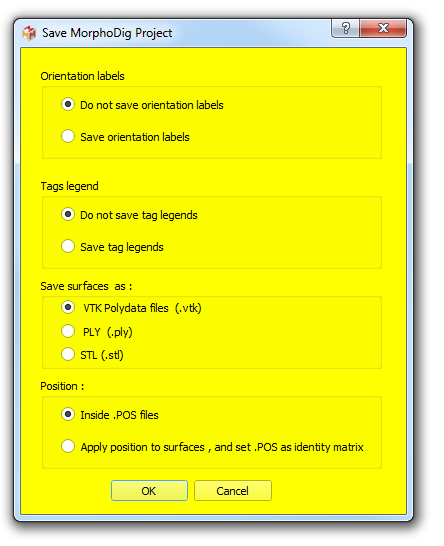
\includegraphics[scale=0.5]{../images/07/project/save_ntw.png}
 \captionof{figure}{Save project window.}
\label{save_project_file}
\end{figure}

The advantage of working with projects is that all involved objects and their properties (surfaces, landmarks, positions etc.) can be reloaded later all at once (and not 1 by 1). 

\subsection{Acknowledgements}
Thanks to the MRI imaging platform for the access to imaging facilities.

%\nocite{*}   % All bibliography items appear without citation in the text

%\cleardoublepage
%\phantomsection

%\addcontentsline{toc}{section}{References}
\section{References}
 \bibliography{Tutorial03}		
\end{document} 

